\documentclass[5pt]{article}
\usepackage{mathptmx,amsmath}
\usepackage{pdfslide2,pause}
\usepackage{eurosym}
\usepackage[portuguese,english]{babel}
\usepackage{kerkis}
\usepackage{colortbl} % used to highlight row or columns of tables. http://www.tug.org/pracjourn/2007-1/mori/mori.pdf
\usepackage[small]{caption} % more option on http://www.dd.chalmers.se/latex/Docs/PDF/caption.pdf
\usepackage[tight,scriptsize]{subfigure}
\usepackage{lastpage}
\usepackage{chngcntr}
\usepackage[absolute,overlay]{textpos}
\usepackage{tabto}
\usepackage{animate}
\usepackage{listings}
\captionsetup{labelformat=empty,skip=-0.8cm}

%\lstset{
%    language=Matlab,                % choose the language of the code
%    basicstyle=\ttfamily\tiny,       % the size of the fonts that are used for the code
%    numbers=none,                   % where to put the line-numbers
%    numberstyle=\tiny,              % the size of the fonts that are used for the line-numbers
%    stepnumber=1,                   % the step between two line-numbers. If it's 1 each line will be numbered
%    numbersep=5pt,                  % how far the line-numbers are from the code
%    backgroundcolor=\color{white},  % choose the background color. You must add \usepackage{color}
%    showspaces=false,               % show spaces adding particular underscores
%    showstringspaces=false,         % underline spaces within strings
%    showtabs=false,                 % show tabs within strings adding particular underscores
%    tab=\rightarrowfill,
%    frame=none,	                    % adds a frame around the code
%    tabsize=2,	                    % sets default tabsize to 2 spaces
%    captionpos=b,                   % sets the caption-position to bottom
%    breaklines=true,                % sets automatic line breaking
%    breakatwhitespace=false,        % sets if automatic breaks should only happen at whitespace
%    title=\lstname,                 % show the filename of files included with \lstinputlisting; also try caption instead of title
%    escapeinside={\%*}{*)},          % if you want to add a comment within your code
%    morekeywords={ifftshift,fftshift},
%    keywordstyle=\bfseries\color[rgb]{0,0,0.3},
%    commentstyle=\color[rgb]{0.133,0.5,0.133}
%}
%\lstset{
%    emph={function,end,for,if,while},
%    emphstyle=\bfseries\color[rgb]{0.6,0,0},
%}

\definecolor{itblue}{rgb}{0.0,0.0,0.5}
\definecolor{itred}{rgb}{0.82,0.18,0.24}
\newcommand{\pageNum}{
    \begin{picture}(0,0)(0,0)
        \put(-15,-390){
            \begin{minipage}{1.8cm}
            \end{minipage}
        }
    \end{picture}
}
\newcommand{\cb}[1]{{\color{itblue} #1}}%
\newcommand{\cred}[1]{{\color{itred} #1}}%
\newcommand{\bb}[1]{{\textbf{\color{itblue} #1}}}%
\newcommand{\br}[1]{{\textbf{\color{itred} #1}}}%
\renewcommand{\labelitemi}{\textcolor{itred}{\normalsize $\bullet$}}
\renewcommand{\labelitemii}{\textcolor{itblue}{$\bullet$}}
\newcommand{\mysection}[1]{\section*{\pageNum\color{itred}\sffamily #1}\vspace*{0.5cm}\overlay{it_1.png}\sffamily}%
\newcommand{\ITfootnote}[1]{\hspace{1.8cm}\begin{minipage}{13cm}\tiny{#1}\end{minipage}}
\newcommand{\edfaGain}{$G=\exp\left(\frac{\alpha}{2}L_{span}\right)$}
\newenvironment{reference}{
    \begin{textblock*}{0.7\textwidth}(32mm,137mm)\tiny\noindent\bgroup\color{black}
}
{
    \egroup\end{textblock*}
}


\graphicspath{{./Figures/}}
\pagestyle{title}

\hyphenpenalty=50000
\tolerance=10000

\setlength{\textheight}{1.5\textheight}

%%%%%%%%%%%%%%%%%%%%%%%%%%%%%%%%%%%%%%%%%%%%%%%%%%%%%%%%%%%%%%%%%%%%%%%%%%%%%%%%%%%%%%%%%%%%%%%%%%%
%%%%%%%%%%%%%%%%%%%%%%%%%%%%%%%%%%%%%%%%%%%%%%%%%%%%%%%%%%%%%%%%%%%%%%%%%%%%%%%%%%%%%%%%%%%%%%%%%%%

\begin{document}

%************************************************************************************************
%                                          SLIDE
%************************************************************************************************
\pagenumbering{roman}
\begin{titlepage}  \overlay{it_0.png}

\color{itblue} \sffamily \noindent \small
\hspace*{1cm}  Universidade de Aveiro\\ %Instituto\\ Superior T�cnico, Instituto de Telecomunica��es\\
\hspace*{1cm}  2018-2019\\ 

\vspace*{1cm}
\begin{center}
    \color{black} \sffamily \noindent \Large
    \br{Coherent One Way (COW) QKD Protocol \\}
\end{center}
\vspace{6mm}
\begin{center}
    \color{black}
    \textbf{João António, Daniel Silva, Armando N. Pinto\\}
    {}
\end{center}

\vspace{0.0mm}
\scriptsize
\begin{center}
Department of Electronics, Telecommunications and Informatics,\\
University of Aveiro, Aveiro, Portugal\\
Instituto de Telecomunica\c{c}\~{o}es, Aveiro, Portugal\\
\end{center}

\vspace{1.0cm}
\hspace*{13.2cm}\tiny \copyright 2005, it - instituto de telecomunica\c{c}\~{o}es\hfill

\end{titlepage}


\renewcommand{\headsep}{-25pt}
\pagenumbering{arabic}

%--------------------------------------------------------------------------------------------------
%------------ SLIDE -------------------------------------------------------------------------------

\mysection{COW - Protocol}\large
\vspace*{1.0cm}

\begin{description}
  \item[Step 1] Alice produces:
      $$|0\rangle = |\alpha\rangle_{2k} |0\rangle_{2k+1},$$
      $$|1\rangle = |0\rangle_{2k} |\alpha\rangle_{2k+1}.$$
      $$|d\rangle = |\alpha\rangle_{2k} |\alpha\rangle_{2k+1}.$$

      where $|0\rangle$ is teh vacuum state and $|\alpha\rangle$ is a coherent state of light with intensity $\mu=|\alpha|^2$.
      
      Alice produces $|d\rangle$ with probability $f$ and the quantum signal cannot be divided bitwise (coherence of the laser).
      
      $$|...0d10...\rangle = |...:0\alpha:\alpha\alpha:\alpha0:0\alpha...\rangle$$

\end{description}

%--------------------------------------------------------------------------------------------------
%------------ SLIDE -------------------------------------------------------------------------------

\mysection{COW - Protocol}\large

\begin{description}
  \item[Step 2] Alice uses an attenuator to around 0.1 photons per pulse and then transmits through a quantum channel.

  \item[Step 3] Bob uses a 90:10 beamsplitter making 90\% of the photons into the SPD{\tiny 1} to arrival time measurements, the remaining 10\% are used to measure phase coherence.
  \begin{figure}[hbt]
    	\centering
    	\includegraphics[width=0.6\textwidth, height=6cm]{./figures/Bob.pdf}
        	\label{bob}
    \end{figure}
\end{description}

%--------------------------------------------------------------------------------------------------
%------------ SLIDE -------------------------------------------------------------------------------

\mysection{COW - Protocol}\large
\vspace*{0.5cm}

In the UMZI (Mach-Zehnder Interferometer) the delayed half of each pulse is recombined in the non-delayed half the next pulse.

For example, the key $|0\rangle|0\rangle|1\rangle|d\rangle|1\rangle|1\rangle |0\rangle|1\rangle$
  \begin{figure}[hbt]
    	\centering
    	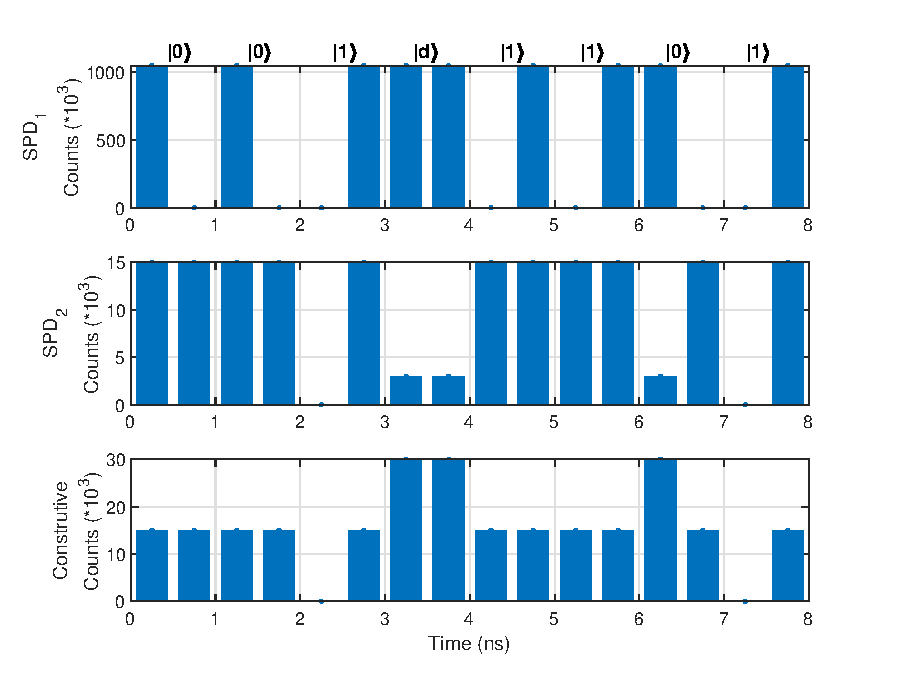
\includegraphics[width=0.75\textwidth, height=8cm]{./figures/DectedSignals.eps}
        	\label{cen}
    \end{figure}

%--------------------------------------------------------------------------------------------------
%------------ SLIDE -------------------------------------------------------------------------------

\mysection{COW - Protocol - Attacks}\large
\vspace*{1cm}
\begin{description}


\item [Step 4]Alice informs Bob when she sent a decoy pulse.

\item [Step 5]They calculate the visibility (V) and the QBER (Q) of the key.
$$ V = \frac{I_{max}-I_{min}}{I_{max}+I_{min}}$$
where the $I_{max}$ and $I_{min}$ are the average pulse intensities for constructive and destructive interference respectively.

They also share a small part of the key in a public channel, to see if there are errors in the message.
\end{description}
\vspace*{1cm}
A loss of coherence and therefore a reduction of the visibility 
reveal the presence of an eavesdropper, in which case the key is simply discarded
%--------------------------------------------------------------------------------------------------
%------------ SLIDE -------------------------------------------------------------------------------
\mysection{COW - Protocol - Attacks}\large
%\vspace*{0.2cm}
\begin{itemize}
\item Beam-splitting attack - Eve removes a small part from the intensity of the original message and send the rest to bob in a no-losses channel (symbolized by a red line). Eve introduces additional errors in order to make her information equal to the Bob information. 
\item Active beam-splitting attack - Eve removes smaller intensities of the message and can make individual measurements and block some of it.

  \begin{figure}[hbt]
    	\centering
    	\includegraphics[width=0.6\textwidth, height=6cm]{./figures/Bob2.pdf}
        	\label{bob2}
    \end{figure}
    


%--------------------------------------------------------------------------------------------------
%------------ SLIDE -------------------------------------------------------------------------------
\mysection{COW - Protocol}\large
\vspace*{1cm}
\item Unambiguous state discrimination (USD) - Alice and Bob only check for coherence in two successive pulses. 
d
So if Eve attacks while they don't check the coherence, she can do an unnoticed attack. But if systematically, they notice that no decoy is detected.
	\begin{table}[hbt]
		\centering
	\begin{tabular}{ll}

	Name  & Discriminating                                     \\
	USD3  & $|0\rangle|\alpha\rangle|0\rangle$                 \\
	USD4a & $|0\rangle|\alpha\rangle:|\alpha\rangle|0\rangle$  \\
	USD4b & $|0\rangle:|\alpha\rangle|\alpha\rangle:|0\rangle$
	\end{tabular}
	\end{table}
\end{itemize}	
%-------------------------------------------------------------------
%------------ SLIDE ------------------------------------------------
\mysection{} \sffamily
\vspace{-10mm}
\large\centerline{E-mail: joaoantonio@ua.pt}


\end{document}
